%% ch02_banking_foundations.tex -- generated from chapter_2_banking_and_financial_services_foundations.md
%% Do not edit by hand; edit the markdown and re-run build_tex.py.

\chapter{Banking and Financial Services Foundations}
\label{chap:ch02_banking_foundations}

\begin{quote}
\textbf{Purpose.} This chapter supplies the business vocabulary needed for the four case studies: credit assessment, financial-document extraction, customer-onboarding KYC/EDD, and investment research and portfolio monitoring. The goal is not to train a banker or provide jurisdiction-specific compliance advice. It is to help a reader recognize what the business is trying to do, what the data represents, who owns a decision, and where an AI system may assist.
\end{quote}
\section*{Learning outcomes}
\addcontentsline{toc}{section}{Learning outcomes}
\label{sec:ch02_banking_foundations-learning-outcomes}

By the end of this chapter, you should be able to:

\begin{enumerate}
\item Place a use case within the relevant part of a financial institution.
\item Describe the lending process from first contact to recovery.
\item Read the basic relationships among financial statements and understand why labels, periods, units, and consolidation matter.
\item Distinguish customer identification, beneficial ownership, source of wealth, source of funds, and screening.
\item Interpret the basic language of private banking, portfolio construction, and portfolio monitoring.
\item Identify decision owners, control points, and audit evidence in an interview-style case study.
\end{enumerate}
\begin{quote}
\textbf{How to use the chapter.} Business terms differ by institution and jurisdiction. The examples below are illustrative, not universal thresholds, accounting rules, legal advice, or investment recommendations. If a later case study describes a scoring threshold, a 25\% ownership rule, or a sample watchlist, read it as that project's configured implementation, not a rule that automatically applies to every bank.
\end{quote}
\medskip\hrule\medskip
\section{Banking Business Overview}
\label{sec:ch02_banking_foundations-2-1-banking-business-overview}

A financial institution moves funds, extends credit, safeguards assets, manages investments, and helps clients meet financial goals. The same customer may interact with several units: a company could have a current account, a working-capital facility, a private-banking relationship for its founder, and an investment-banking mandate. That is why a case-study solution must ask which business process and decision it supports.

\subsection{Retail banking}

Retail banking serves individuals and households. Common products include transaction accounts, deposits, cards, mortgages, personal loans, and payments. Typical operational questions are: Is the applicant the person they claim to be? Can they repay a loan? Does a transaction look suspicious? Which customer documents are still missing?

\textbf{Example.} A customer applying for a mortgage provides identification and proof of income. Document extraction can help populate an application, but policy checks, affordability calculations, and approval authority remain separate concerns.

\subsection{Corporate and commercial banking}

Corporate and commercial banking serves businesses, from smaller enterprises to large groups. Products may include term loans, revolving credit, trade finance, cash management, and guarantees. Analysts examine audited accounts, debt schedules, cash flows, collateral, covenants, and the purpose of borrowing. A corporate credit memo is a decision-support document for the credit process, not a customer-facing marketing summary.

\textbf{Example.} A manufacturer requests an additional working-capital line. The analyst must ask whether sales growth is supported by cash collection, whether debt service is affordable, and whether any existing covenant has been breached. The credit-assessment case study lives primarily here.

\subsection{Private banking and wealth management}

Private banking supports clients with complex assets, financial structures, or tailored service needs. Wealth management focuses on investments, asset allocation, suitability, and long-term goals. A relationship manager gathers a client's circumstances and investment objectives, but onboarding, sanctions, suitability, and portfolio decisions still require distinct controls.

\textbf{Example.} A founder who sold a business may need to demonstrate how the wealth was generated, why an offshore holding company appears in the ownership chain, and whether a proposed concentrated equity portfolio fits their ability and willingness to bear losses. The KYC and investment-copilot case studies connect to this domain.

\subsection{Investment banking}

Investment banking commonly covers advisory and capital-markets activity: mergers and acquisitions, securities issuance, underwriting, and related institutional services. Investment banking is not synonymous with investment portfolio management. A capital-raising advisory mandate and a private client's model portfolio involve different counterparties, data, permissions, and regulations.

\subsection{Lending institutions and NBFCs}

Lending institutions may specialize in consumer, SME, vehicle, housing, or business credit. In India, a non-banking financial company, or NBFC, is a defined category of company principally engaged in specified financial activities, including lending; its licensing and deposit-taking position should not be assumed to match a bank's. The Reserve Bank of India's FAQ is the appropriate starting point for the local definition.

\subsection{Fintech platforms}

Fintech platforms use software to deliver or enable services such as digital onboarding, payments, lending, brokerage, and financial data aggregation. A fintech may serve customers directly or provide technology to a regulated institution. In either case, clarify which organization owns the customer relationship, the regulated activity, the data, and the final decision.

\subsection{Banks, customers, regulators, and service providers}

\begin{figure}[htbp]
\centering
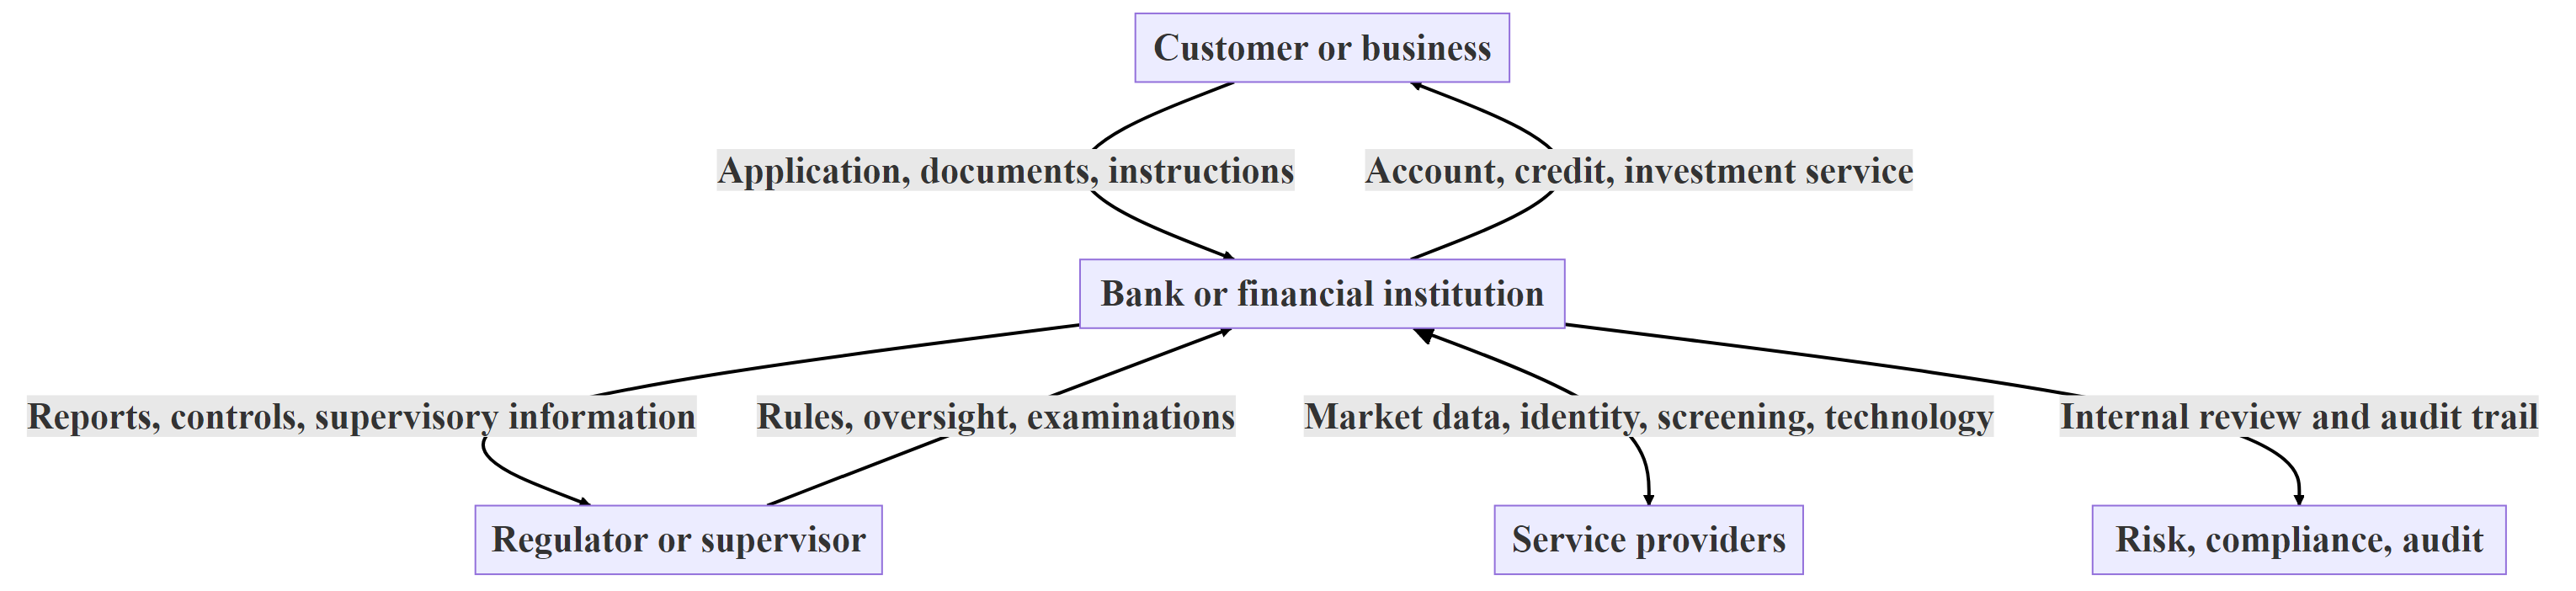
\includegraphics[width=\textwidth,height=0.85\textheight,keepaspectratio]{../diagrams/chapter_2_banking_foundations/01_flowchart_banks-customers-regulators-and-service-providers.png}
\caption{Banks, customers, regulators, and service providers}
\label{fig:ch02_banking_foundations-01-flowchart-banks-customers-regulators-and-service-providers}
\end{figure}

A data vendor can supply a market quote or screening candidate; it does not become the bank's credit approver. A model can draft a memo; it does not become the regulated institution's accountable officer. The distinction between supplier, operator, reviewer, and decision-maker underlies every case study. Credit-risk governance guidance emphasizes sound granting, administration, monitoring, and controls.

\textbf{Suggested image:} A swimlane showing one corporate customer interacting with relationship management, credit risk, KYC operations, portfolio services, and a regulator. It would help readers see why a single customer can generate several separate cases and approval workflows.

\medskip\hrule\medskip
\section{Credit and Lending Lifecycle}
\label{sec:ch02_banking_foundations-2-2-credit-and-lending-lifecycle}

Credit is a promise to provide funds or take exposure now in exchange for repayment under agreed terms. The credit lifecycle extends well beyond an initial score: the lender must understand the customer, decide whether and how to lend, document the obligation, and monitor it. The Basel Committee's current credit-risk principles explicitly cover sound credit granting, administration, measurement, monitoring, and controls.

\begin{figure}[htbp]
\centering
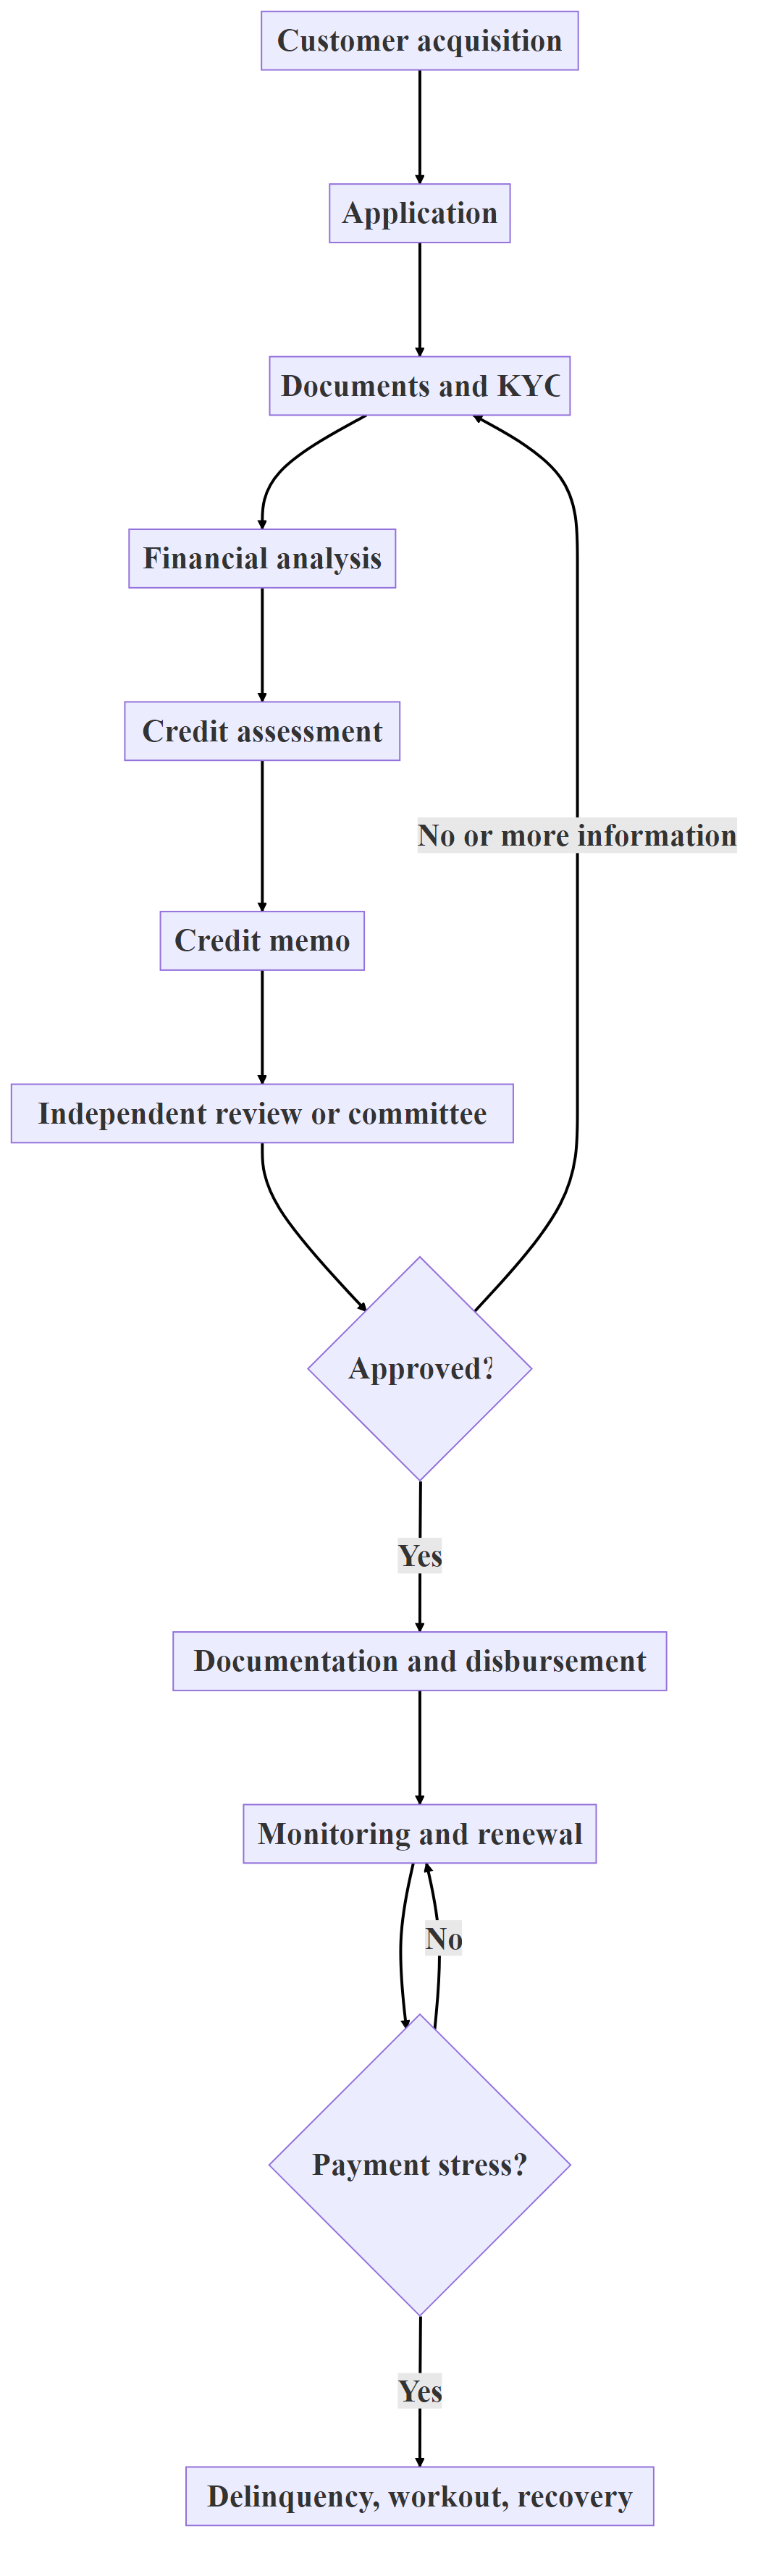
\includegraphics[width=\textwidth,height=0.85\textheight,keepaspectratio]{../diagrams/chapter_2_banking_foundations/02_flowchart_2-2-credit-and-lending-lifecycle.png}
\caption{Credit and Lending Lifecycle}
\label{fig:ch02_banking_foundations-02-flowchart-2-2-credit-and-lending-lifecycle}
\end{figure}

\subsection{Customer acquisition and application}

Acquisition begins when a relationship manager or digital channel identifies a customer's financing need. The application describes the borrower, requested amount, facility type, purpose, tenure, existing obligations, and intended repayment source. These are related but different: a loan's \textit{purpose} might be inventory purchase; its \textit{repayment source} might be operating cash flow.

\textbf{Example.} A business requests a 12-month revolving facility to finance receivables. An interviewer should ask whether the system is assessing a new customer, renewing an existing line, or increasing exposure; each has a different evidence and history requirement.

\subsection{Document collection}

Typical business-lending documents include audited financial statements, interim accounts, bank statements, debt schedules, ownership documents, tax records, collateral evidence, facility letters, and covenant certificates. Documents are not interchangeable. An audited annual report can establish historical figures; a current debt schedule may better reflect the borrower's near-term maturities.

\textbf{Agent role:} locate clauses and extract line items with source pages. \textbf{Code role:} reject invalid files, normalize units, check missing required documents, calculate figures, and enforce required-field rules.

\subsection{Financial analysis and credit assessment}

Financial analysis asks whether the business generates enough cash, has an appropriate leverage level, can meet interest and principal obligations, and has adequate liquidity. Credit assessment also considers management quality, business model, sector, collateral, ownership, legal risks, and adverse information. A credit rating or score summarizes policy-defined risk factors; it does not replace the underlying evidence.

A credit memo usually records the borrower and facility, historical results, ratios, repayment analysis, strengths, risks, mitigants, proposed structure, covenants, exceptions, and recommendation. A model may draft prose, but critical values and decision thresholds should be computed and checked independently.

\subsection{Review, approval, and disbursement}

A credit officer or committee reviews the memo, the policy exceptions, and any proposed conditions. Approval may be conditional on additional documentation, security registration, or revised terms. Disbursement occurs only after the lender confirms the required documents and conditions are satisfied. A draft recommendation is not an approval.

\subsection{Monitoring, renewal, delinquency, and recovery}

After lending, the institution tracks repayments, covenant compliance, updated financials, collateral, sector developments, and early warning signals. Renewal revisits the risk when a facility matures or requires extension. Delinquency means scheduled obligations have not been met; recovery or workout focuses on resolving the exposure through repayment plans, restructuring, collateral enforcement, or other authorized processes.

\textbf{Example.} A borrower was profitable at approval but later shows weakening cash collections and rising debt. The monitoring workflow should flag the change even if last year's ratio looked acceptable. A system that produces a memo once but ignores the life of the facility does not cover the full credit problem.

\medskip\hrule\medskip
\section{Financial Statements}
\label{sec:ch02_banking_foundations-2-3-financial-statements}

A company's statements answer three different questions: What does it own and owe at a date? How much did it earn over a period? Where did cash come from and go over that period? The SEC's introduction distinguishes balance sheets as point-in-time snapshots and income and cash-flow statements as period flows.

\subsection{Balance sheet}

The balance sheet reports assets, liabilities, and equity at a particular reporting date. The accounting identity is:

\[
\text{Assets} = \text{Liabilities} + \text{Equity}
\]

For a simplified company with assets of 1,000 and liabilities of 650, equity is 350, all in the same currency and unit. This is a consistency check, not a claim that accounting balance proves the company is solvent or liquid. A firm may own illiquid assets while short-term obligations are due soon.

\subsection{Income statement}

The income statement reports revenue, expenses, and profit over a period. Revenue is not cash collected; profit is not cash in the bank. A business can report strong sales while customers have not yet paid. Interest expense matters to lenders because it reduces capacity to service debt.

\subsection{Cash-flow statement}

The cash-flow statement organizes cash movements into operating, investing, and financing activities. Operating cash flow indicates whether day-to-day business activity generates cash. Investing cash flow includes purchases or sales of long-term assets; financing cash flow includes borrowing, repayment, and capital flows. A business can be profitable but experience cash stress if receivables rise or inventory absorbs working capital.

\subsection{Notes, schedules, and disclosures}

Notes explain accounting policies, borrowings, maturity profiles, contingencies, guarantees, related-party transactions, segment information, and other context not visible in headline numbers. Schedules break aggregate figures into components. An apparently healthy leverage ratio may need qualification if guarantees, litigation, or a going-concern warning appear in the notes. Notes must be linked to the specific statement, period, and source page.

\subsection{Ratios and indicators}

Ratios are calculated from extracted figures; their definitions should be recorded, not guessed from a label. Common examples include:

\begin{xltabular}{\textwidth}{>{\raggedright\arraybackslash}X >{\raggedright\arraybackslash}X >{\raggedright\arraybackslash}X >{\raggedright\arraybackslash}X}
\caption{Ratios and indicators}\label{tab:ch02_banking_foundations-ratios-and-indicators-1}\\
\hline
\textbf{Indicator} & \textbf{Simplified formula} & \textbf{Question it helps answer} & \textbf{Important caveat} \\
\hline
\endfirsthead
\caption[]{Ratios and indicators (continued)}\\
\hline
\textbf{Indicator} & \textbf{Simplified formula} & \textbf{Question it helps answer} & \textbf{Important caveat} \\
\hline
\endhead
Current ratio & Current assets $\div$ current liabilities & Can near-term assets cover near-term liabilities? & Inventory and receivables may be hard to realize \\
Debt-to-equity & Interest-bearing debt $\div$ equity & How levered is the capital structure? & Some sources use total liabilities instead of debt; specify definition \\
EBITDA margin & EBITDA $\div$ revenue & How much operating earnings are generated per unit of sales? & EBITDA is not operating cash flow \\
Interest coverage & EBIT $\div$ interest expense & Can earnings cover interest? & Denominator and period must be consistent \\
Operating cash flow to debt & Operating cash flow $\div$ total debt & How does cash generation compare with indebtedness? & A single year can be distorted by working capital \\
\hline
\end{xltabular}

\textbf{Example.} If current assets are 240 and current liabilities are 120, the current ratio is 2.0. If those figures came from different periods, currencies, or consolidation scopes, the arithmetic may be correct but the analysis invalid. The SEC notes that ratios must be read alongside the statements and that desirable values vary by industry.

\subsection{Consolidated versus standalone statements}

A consolidated statement presents a parent and its subsidiaries as a single economic entity; a separate or standalone statement describes the reporting entity on its own basis. These figures are not interchangeable. A document-extraction system must preserve the column header and entity scope rather than indiscriminately selecting the largest number. IFRS defines consolidated reporting at the group level and describes elimination of intragroup items.

\subsection{Fiscal periods and comparative figures}

A balance sheet may report a point in time, such as June 30, 2026, alongside June 30, 2025. An income statement may compare six months ended June 30, 2026 with the corresponding six months in 2025. A flow reported for six months should not be compared directly to a full-year figure without an explicit analytical adjustment. Financial-document systems should store \texttt{period\_end}, period duration or type, currency, scale, statement type, and consolidated/standalone scope per cell.

\begin{figure}[htbp]
\centering
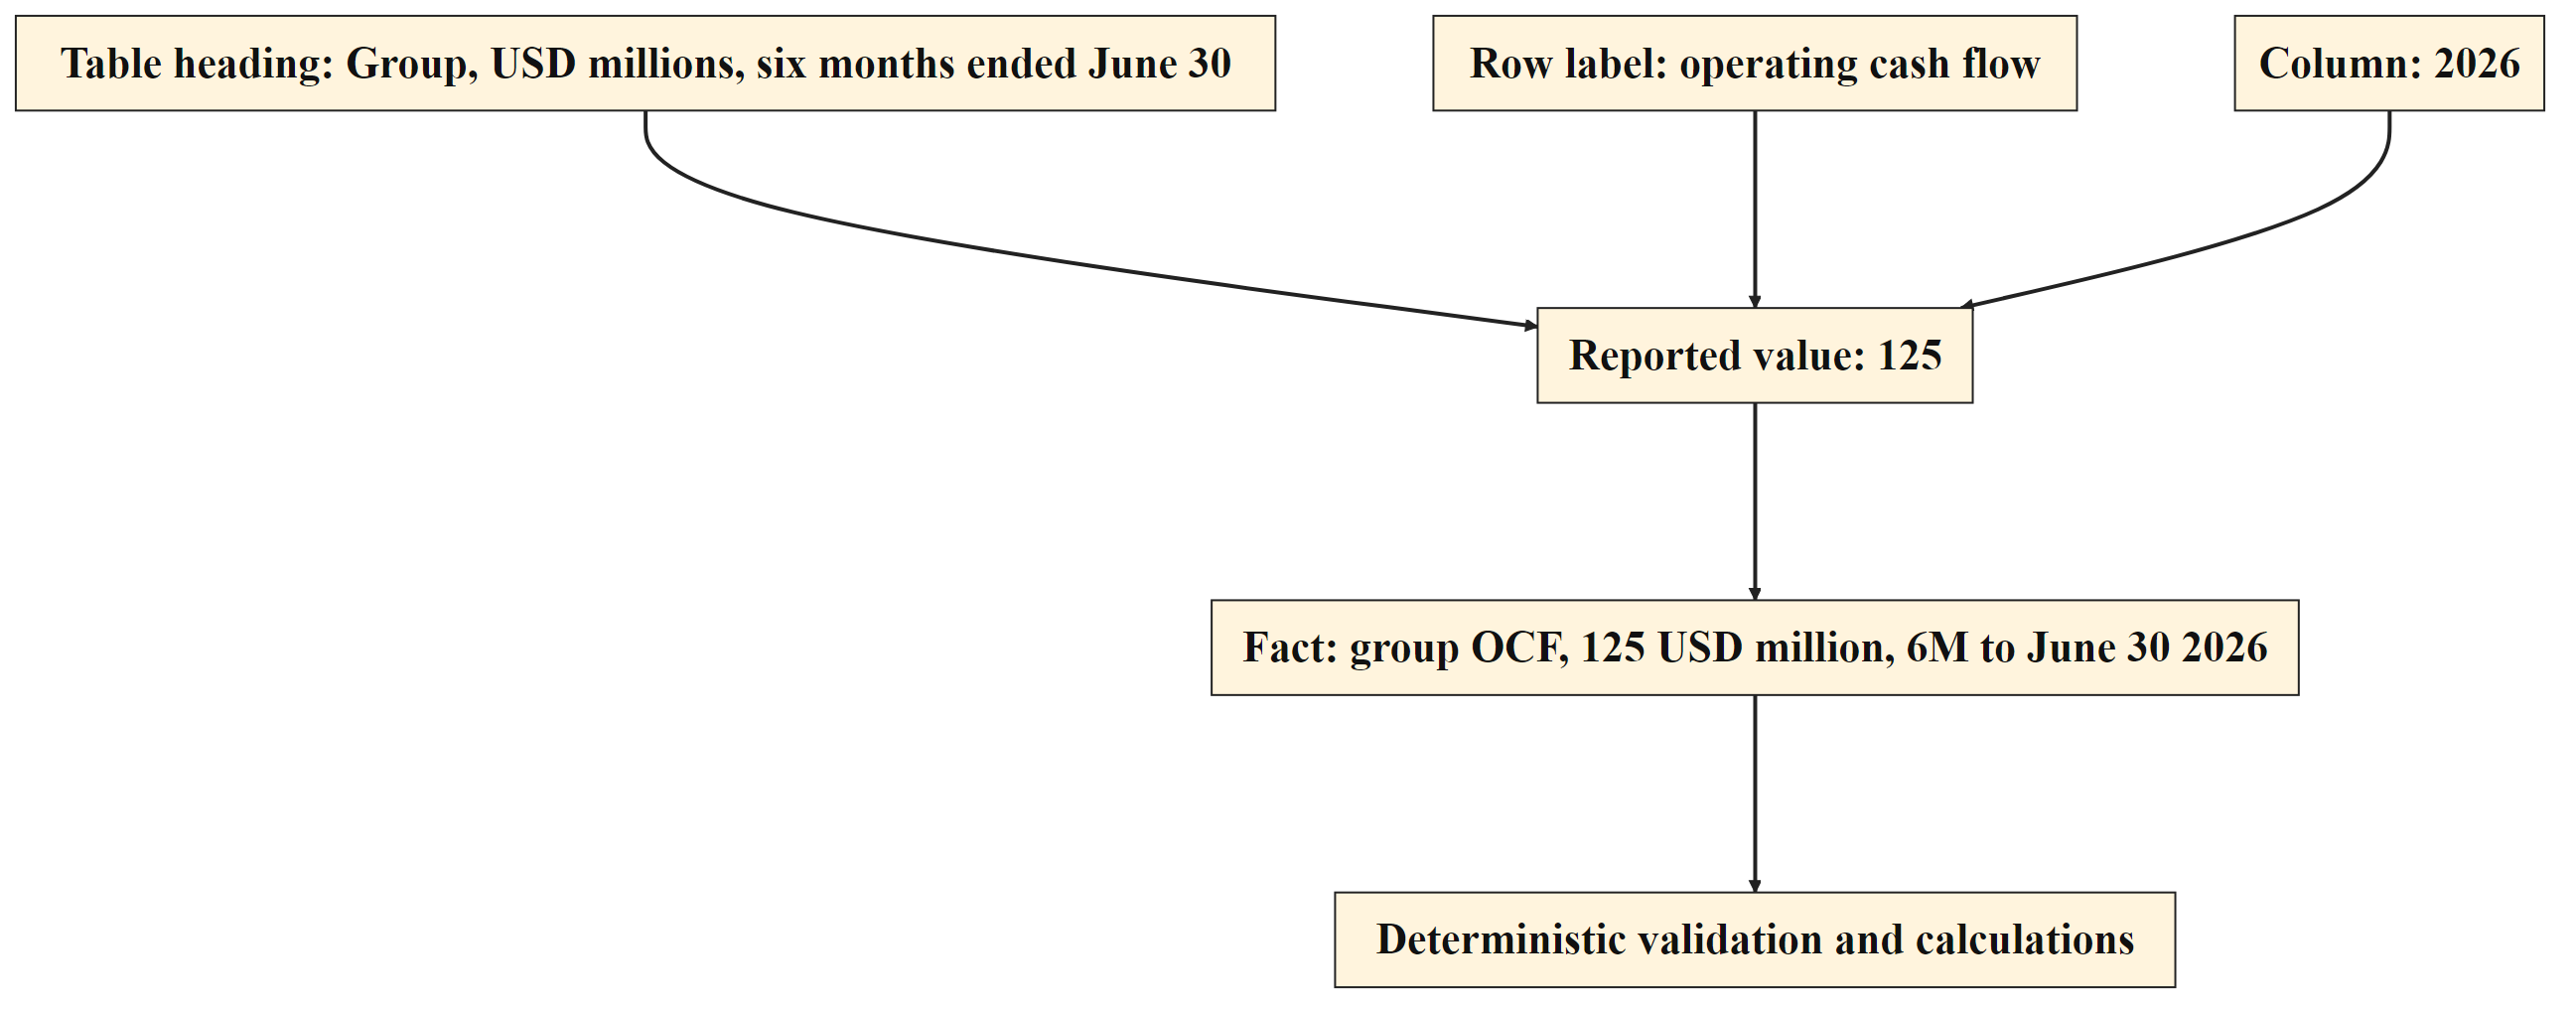
\includegraphics[width=\textwidth,height=0.85\textheight,keepaspectratio]{../diagrams/chapter_2_banking_foundations/03_flowchart_fiscal-periods-and-comparative-figures.png}
\caption{Fiscal periods and comparative figures}
\label{fig:ch02_banking_foundations-03-flowchart-fiscal-periods-and-comparative-figures}
\end{figure}

\textbf{Suggested image:} A marked-up annual-report page with arrows to statement name, currency and scale, comparative-period headers, consolidated column, row label, and footnote. This makes clear why a number without its coordinates is not yet a usable financial fact.

\medskip\hrule\medskip
\section{KYC, AML, and Customer Due Diligence}
\label{sec:ch02_banking_foundations-2-4-kyc-aml-and-customer-due-diligence}

Know your customer, or KYC, is a common operational label for understanding and verifying a customer. Anti-money-laundering controls, or AML controls, address risks that financial services are misused to handle illicit funds. Customer due diligence, or CDD, includes identification and verification, understanding beneficial ownership and the relationship's purpose, and ongoing scrutiny. FATF sets out these elements as part of its international AML/CFT standard, while actual local obligations depend on jurisdiction and institution.

\subsection{Customer identification}

Identify the customer and verify identity with reliable, independent evidence. For a person, this may involve name, date of birth, identification documents, and address. For a legal entity, it may involve registration records, directors, authorized signatories, and the persons who ultimately own or control it. An uploaded identity document is evidence to be checked, not proof that every extracted field is accurate.

\subsection{Beneficial ownership}

A beneficial owner is a natural person who ultimately owns or controls the customer under applicable rules. The institution may need to understand a chain of companies, a trust arrangement, voting rights, or other forms of control. Some case-study implementations use a 25\% threshold as a configurable example; real legal thresholds and control tests must be taken from the applicable regime. FATF's CDD framework explicitly calls for identifying the beneficial owner and understanding legal-person ownership and control structures.

\textbf{Example.} Maya owns 60\% of Holding A, and Holding A owns 50\% of Customer B. Maya's indirect economic ownership through that path is 30\% (0.60 $\times$ 0.50). An ownership graph can calculate this deterministically. A model may extract the two ownership statements from a deed, but it should not be entrusted with the final arithmetic.

\subsection{Source of wealth and source of funds}

\textbf{Source of wealth} explains how a person accumulated overall assets over time: for example, salary, inheritance, or sale of a business. \textbf{Source of funds} explains the origin of the money used for a particular transaction or account funding event. A credible business-sale narrative does not, by itself, verify that the wire arriving next Tuesday came from the sale proceeds. The distinction is particularly important for complex private-banking customers. FATF's PEP measures include reasonable steps to establish both.

\subsection{PEP, sanctions, and adverse media}

A politically exposed person, or PEP, is associated with prominent public functions; relevant checks can extend to family members and close associates. A PEP indication is a risk-management trigger, not a finding of wrongdoing. Sanctions screening checks a person or entity against applicable restrictive lists; a name-similarity candidate is not automatically a confirmed match. Adverse-media checks look for potentially relevant negative public reports; an allegation must be distinguished from an established fact and matched to the right person. FATF Recommendation 12 describes additional measures for foreign PEPs, including senior-management approval, source-of-wealth and source-of-funds measures, and enhanced monitoring.

\subsection{Risk classification and enhanced due diligence}

CDD is risk-based. A relationship may require enhanced due diligence, or EDD, because of PEP status, geography, unusual ownership, opaque source of wealth, transaction behavior, or other factors. EDD can involve more evidence, senior approval, and closer ongoing monitoring; it is not simply a higher score printed on a screen. A rule-based system can calculate configured triggers, while a reviewer determines whether evidence and local policy support the next action.

\subsection{Periodic review}

KYC does not end at account opening. Relationships, addresses, directors, ownership, funding patterns, and risk exposure change. Review frequency and scope should follow applicable rules and risk policies. A historical KYC view is useful only if each version shows what was known at the time, which evidence was used, what changed, and who approved the outcome. FATF calls for ongoing due diligence and application to existing customers when appropriate.

\begin{figure}[htbp]
\centering
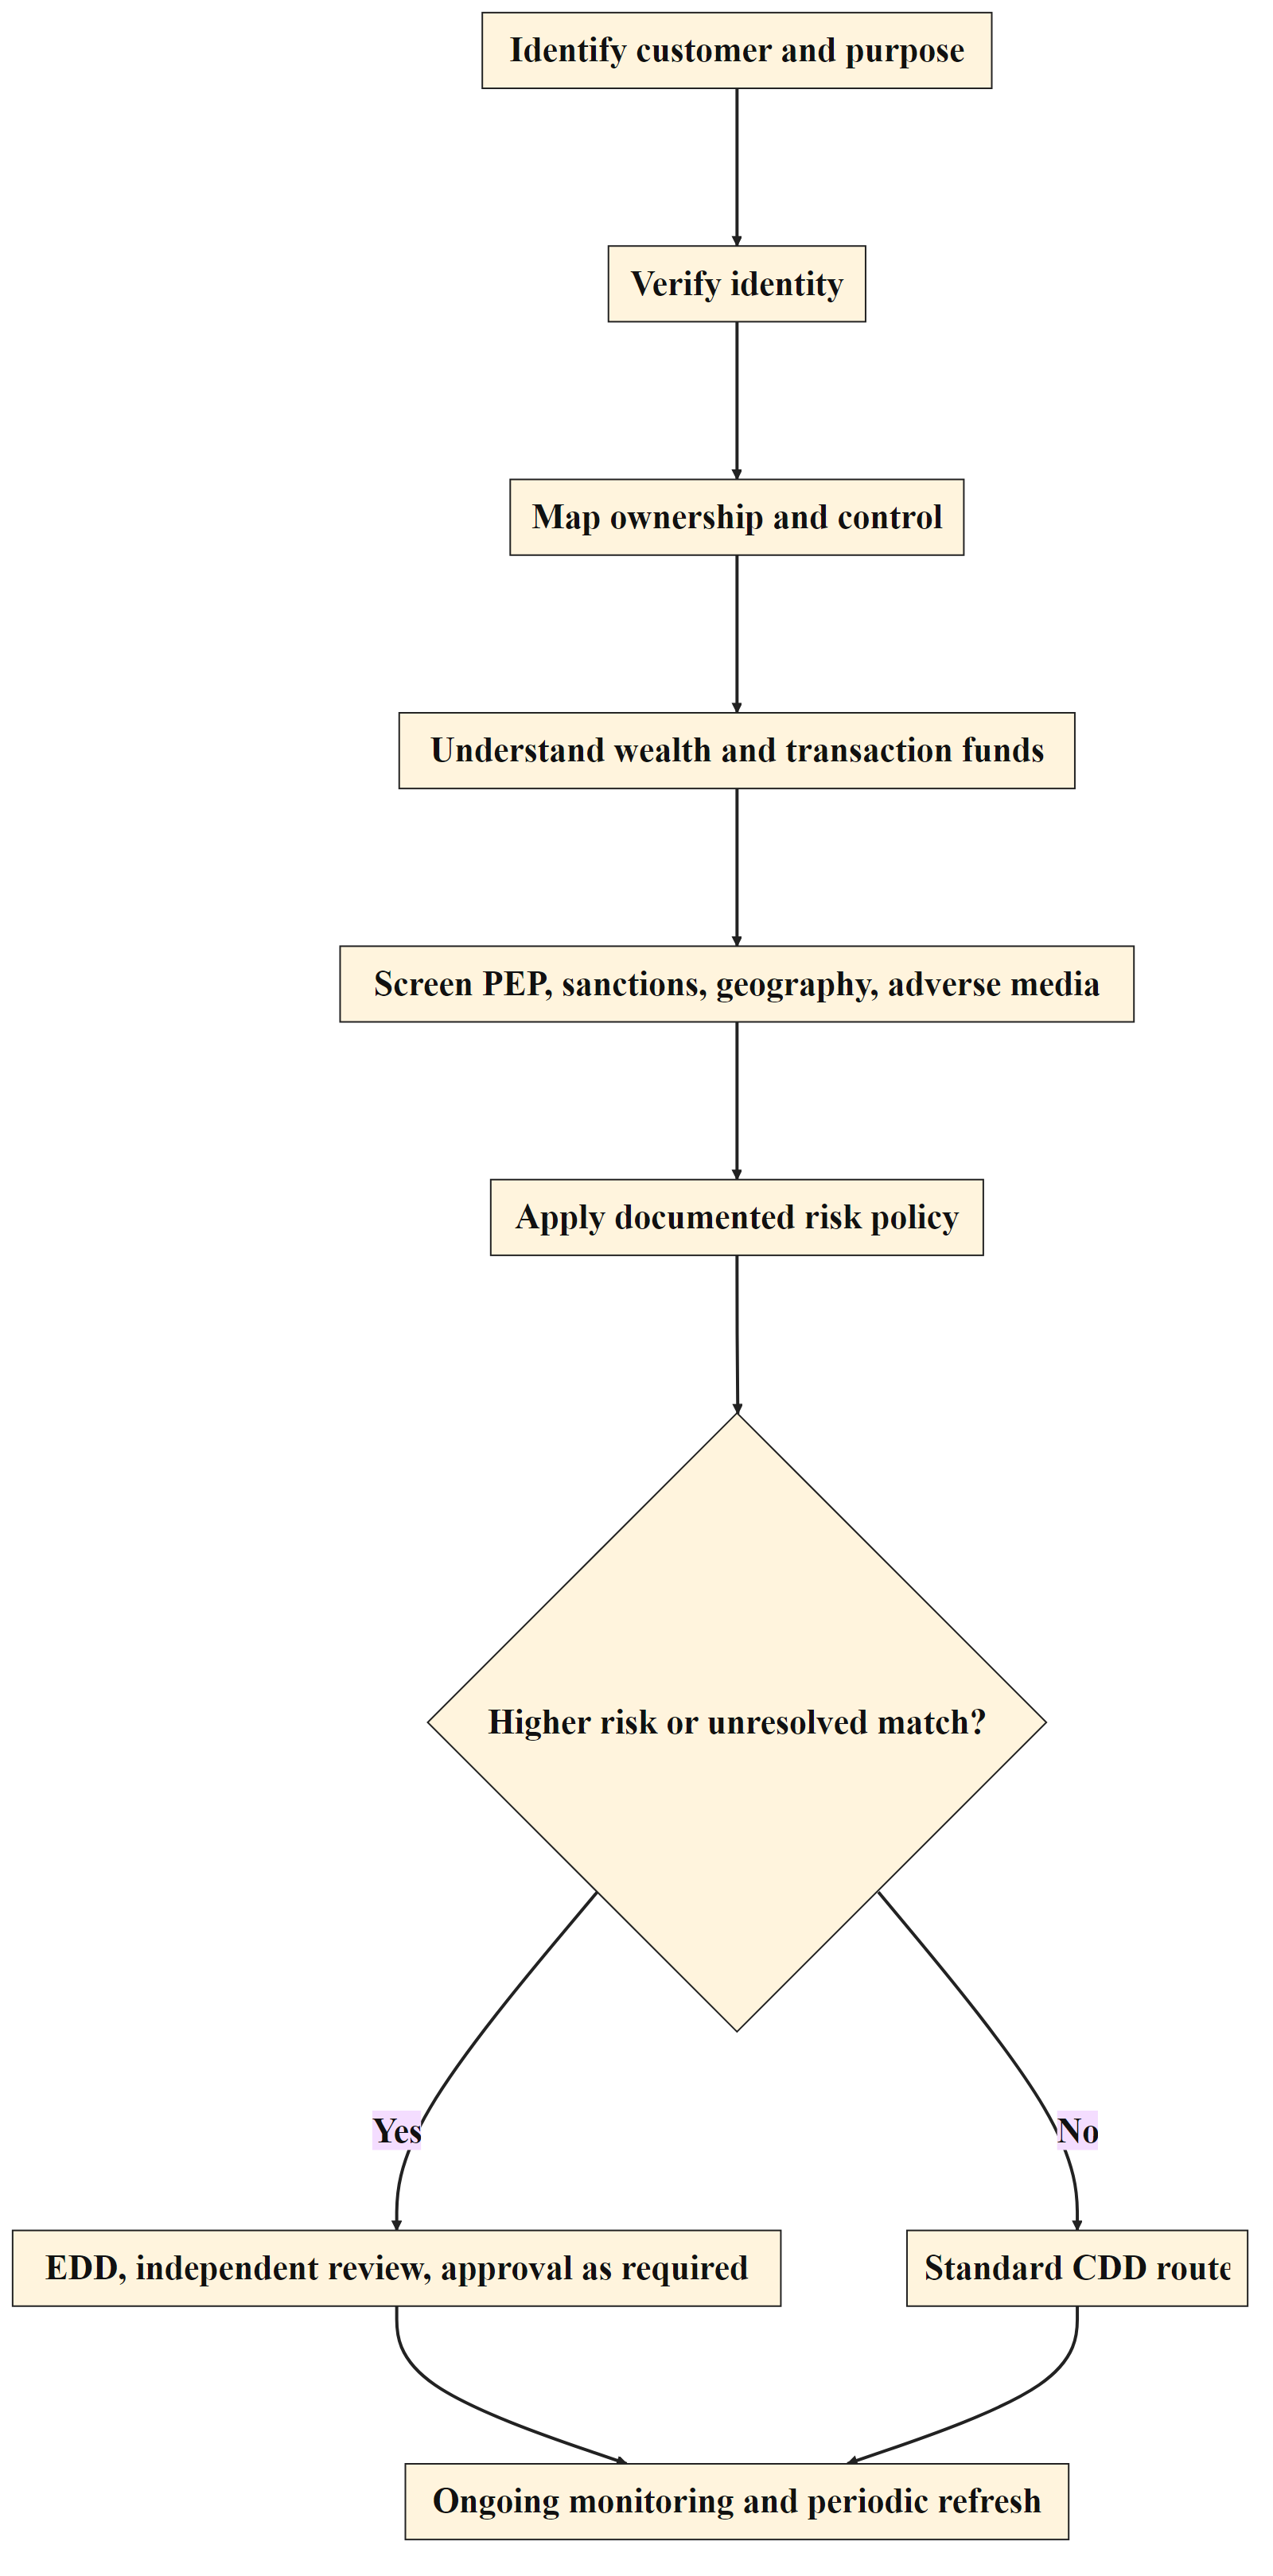
\includegraphics[width=\textwidth,height=0.85\textheight,keepaspectratio]{../diagrams/chapter_2_banking_foundations/04_flowchart_periodic-review.png}
\caption{Periodic review}
\label{fig:ch02_banking_foundations-04-flowchart-periodic-review}
\end{figure}

\textbf{Suggested image:} A simple ownership chart that includes a company, an intermediate holding company, and two natural persons; show economic ownership paths and a separate control role such as trustee. This helps distinguish ``owns 30\%'' from ``controls through a legal role.''

\medskip\hrule\medskip
\section{HNI and Private Banking}
\label{sec:ch02_banking_foundations-2-5-hni-and-private-banking}

High-net-worth individuals, or HNIs, and ultra-high-net-worth individuals, or ultra-HNIs, may have substantial and complex assets. There is no single globally applicable monetary threshold for these terms; institutions define segments for their own services. The practical design implication is complexity: multiple entities, jurisdictions, concentrated holdings, illiquid assets, family structures, and tailored investment objectives.

\subsection{Relationship manager and specialist roles}

The relationship manager coordinates client needs and information gathering. Investment advisers or portfolio managers address portfolio design; compliance performs onboarding and screening; credit teams assess lending against assets or cash flows. One professional may introduce a client, but that does not mean they may clear sanctions, override suitability, or approve a loan.

\subsection{Net worth, liquidity, and cash flow}

Net worth is assets minus liabilities, measured as of a date with valuation assumptions. It is not the same as liquid cash. A founder may have a large private-company stake but little immediately available cash. Liquidity analysis asks how quickly assets can meet near-term needs; cash-flow analysis asks when income, distributions, expenses, debt service, and capital calls occur.

\textbf{Example.} A customer reports assets worth 50 million, including a 45 million private-company stake and 5 million liquid investments. A proposal to fund a 10 million obligation in one month cannot assume the company stake is immediately saleable. Asset classification and valuation evidence are essential.

\subsection{Objectives, risk appetite, and suitability}

Investment objectives might include capital preservation, income, growth, or liquidity for a future payment. \textbf{Risk tolerance} concerns willingness to endure losses; \textbf{risk capacity} concerns the financial ability to absorb them. Time horizon, expected withdrawals, taxes, legal restrictions, and knowledge of products also shape suitability. A model can summarize a client interview; documented policy and authorized advisers must determine whether a proposal is suitable.

\subsection{Concentration and exposure risk}

A portfolio can look diversified by ticker count yet be concentrated in one business, family company, sector, geography, currency, or underlying risk factor. An HNI who earned wealth from a technology company and holds a portfolio heavily weighted toward technology may have a larger combined exposure than the investment account alone suggests. The investment case study's sector and single-name caps are examples of guardrails; they are not universal suitability rules.

\medskip\hrule\medskip
\section{Investments and Portfolio Management}
\label{sec:ch02_banking_foundations-2-6-investments-and-portfolio-management}

An investment portfolio is a collection of holdings held for defined objectives. Portfolio design starts with the client's constraints and risk capacity, not with a list of fashionable securities. Asset allocation, diversification, and rebalancing are core ideas in investor education.

\subsection{Main asset categories}

\begin{xltabular}{\textwidth}{>{\raggedright\arraybackslash}X >{\raggedright\arraybackslash}X >{\raggedright\arraybackslash}X}
\caption{Main asset categories}\label{tab:ch02_banking_foundations-main-asset-categories-2}\\
\hline
\textbf{Category} & \textbf{What the investor generally holds} & \textbf{Main considerations} \\
\hline
\endfirsthead
\caption[]{Main asset categories (continued)}\\
\hline
\textbf{Category} & \textbf{What the investor generally holds} & \textbf{Main considerations} \\
\hline
\endhead
Equities & Ownership interest in a company & Business growth, valuation, volatility, dividends, concentration \\
Bonds / fixed income & Debt claim on issuer & Credit risk, interest-rate sensitivity, maturity, coupons, liquidity \\
Mutual funds & Pooled investments managed under a mandate & Holdings, fees, manager/process, liquidity terms \\
ETFs & Exchange-traded pooled funds & Underlying index or strategy, liquidity, tracking, costs \\
Cash and deposits & Liquid balances or cash-like instruments & Liquidity, inflation, counterparty and currency considerations \\
Alternatives & Assets or strategies outside traditional stocks and bonds & Valuation, liquidity, complexity, correlation, fees \\
\hline
\end{xltabular}

An ETF is a wrapper, not automatically a separate asset class: an equity ETF contributes equity exposure. A bond fund contributes fixed-income exposure even if held as one ticker. Classification should reflect economic exposure rather than file format or product name alone.

\subsection{Asset allocation and diversification}

Asset allocation sets target shares for broad classes. Diversification distributes exposure within and across classes to limit dependence on any one holding or risk. A balanced illustrative mandate might target 55\% equity, 35\% fixed income, 5\% cash, and 5\% alternatives. A target is not a guarantee of return or a substitute for knowing the client's circumstances. The SEC describes allocation as division among categories and diversification as spreading investments to reduce risk.

\subsection{Risk and return}

Return includes price changes and income over a specified period. Risk can mean price volatility, permanent loss, credit default, illiquidity, concentration, or failure to meet a client's spending goal. A high expected return does not prove suitability. Different risk measures answer different questions: volatility describes variability; drawdown describes a decline from a previous peak; concentration describes how much depends on a few positions.

\subsection{Rebalancing}

Weights move as prices change. Rebalancing brings a portfolio toward target allocation by selling overweight holdings, buying underweight ones, or directing new contributions toward underweights. The decision should account for bands, costs, taxes, liquidity, and authorization. A monitoring system may propose trades only when a sleeve breaches its allowed band; it should not execute them simply because the model wrote a persuasive explanation.

\textbf{Example.} A 1,000,000 portfolio has 680,000 in equity, so the equity weight is 68\%. If the target is 55\% with a $\pm$5 percentage-point band, equity exceeds the 60\% upper limit. A simplified move back to target would sell 130,000 of equity, assuming unchanged total value and ignoring transaction costs, taxes, cash flows, and market movements. This is a deterministic proposal for review, not an order to trade.

\subsection{Constraints and benchmarking}

Constraints may include maximum single-name weight, sector cap, prohibited securities, permitted countries, minimum liquidity, investment horizon, and mandate-specific asset mix. A benchmark is a reference used to assess performance or risk in context; the appropriate benchmark depends on what the portfolio is intended to do. Comparing a conservative income portfolio with a growth-equity index alone would be misleading.

\begin{figure}[htbp]
\centering
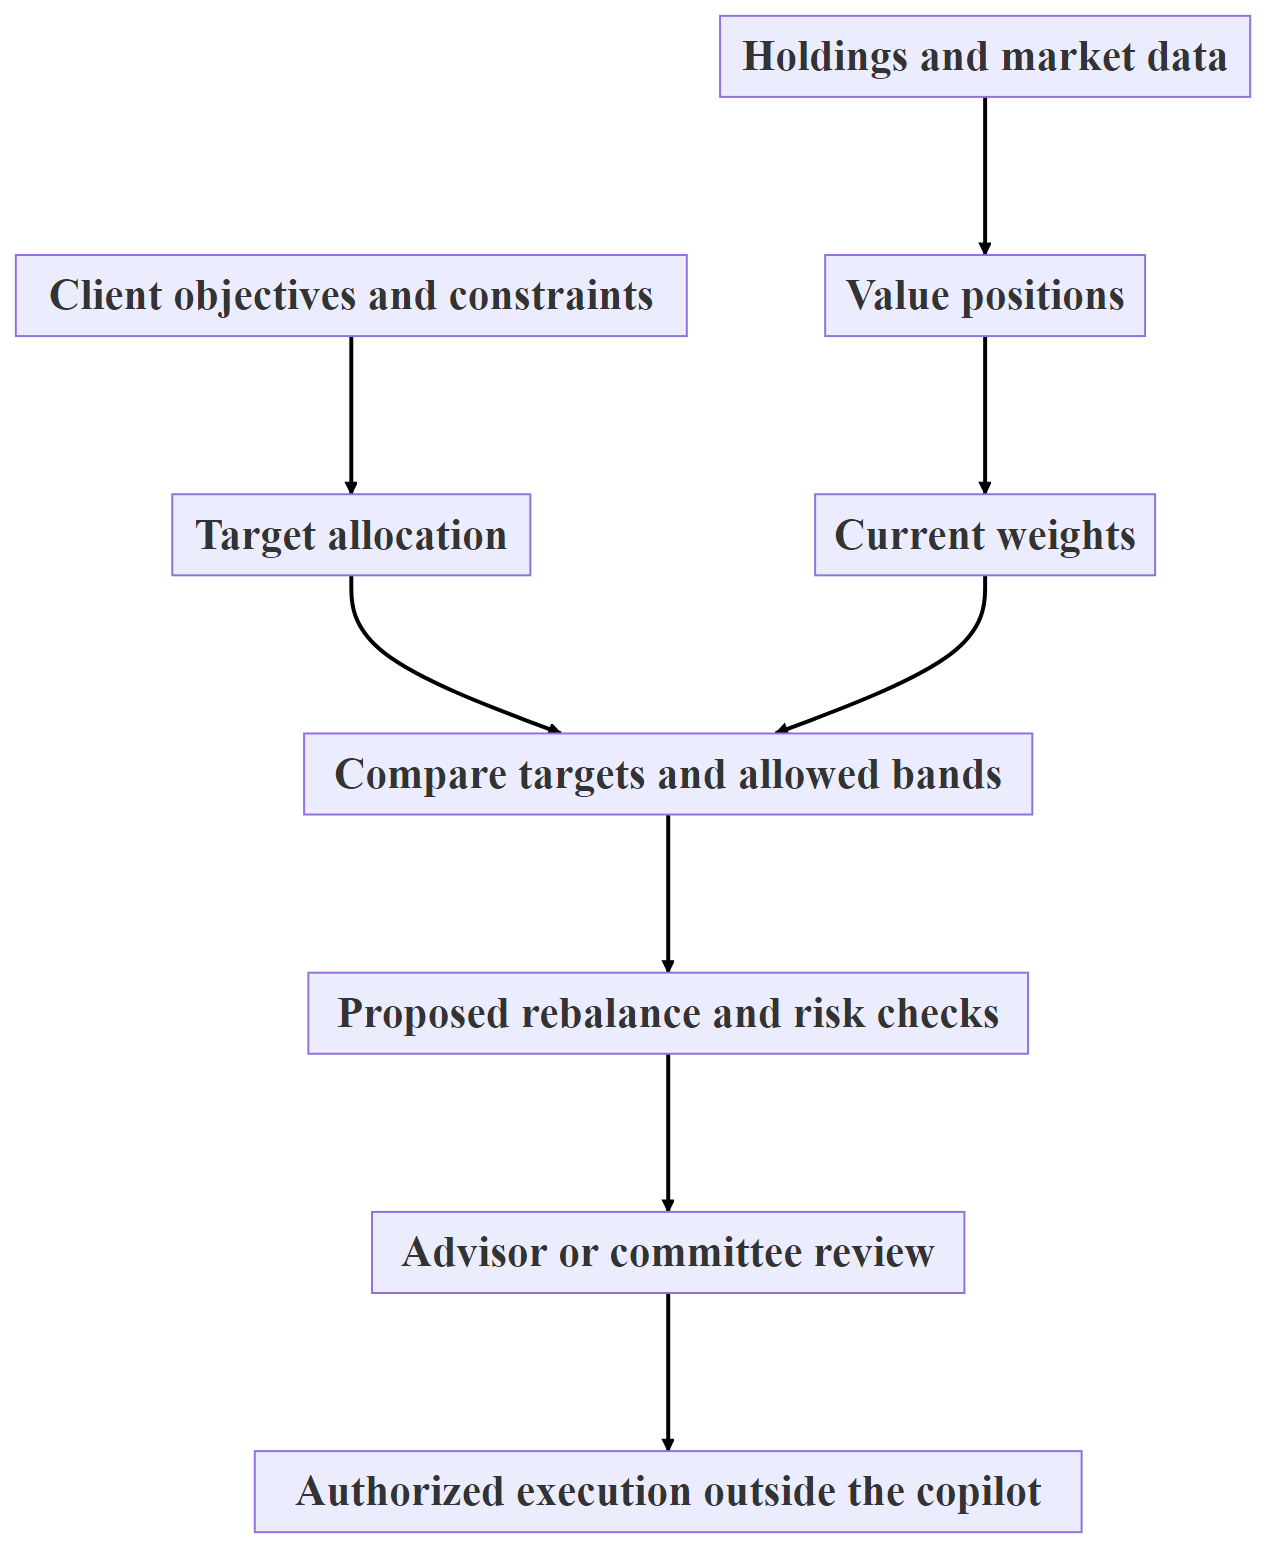
\includegraphics[width=\textwidth,height=0.85\textheight,keepaspectratio]{../diagrams/chapter_2_banking_foundations/05_flowchart_constraints-and-benchmarking.png}
\caption{Constraints and benchmarking}
\label{fig:ch02_banking_foundations-05-flowchart-constraints-and-benchmarking}
\end{figure}

\textbf{Suggested image:} A before-and-after stacked bar chart comparing actual asset mix with target mix, with tolerance bands and a marked equity breach. It would make ``drift'' and ``rebalance'' immediately intuitive.

\medskip\hrule\medskip
\section{Risk, Compliance, and Governance}
\label{sec:ch02_banking_foundations-2-7-risk-compliance-and-governance}

``Risk'' is not one number. A system should identify which risk it is measuring and whose decision it supports. A credit-risk score is not a portfolio-health score; a suspicious-name match is not evidence of credit default.

\begin{xltabular}{\textwidth}{>{\raggedright\arraybackslash}X >{\raggedright\arraybackslash}X >{\raggedright\arraybackslash}X}
\caption{Risk, Compliance, and Governance}\label{tab:ch02_banking_foundations-2-7-risk-compliance-and-governance-3}\\
\hline
\textbf{Risk} & \textbf{Plain-language meaning} & \textbf{Illustrative control or signal} \\
\hline
\endfirsthead
\caption[]{Risk, Compliance, and Governance (continued)}\\
\hline
\textbf{Risk} & \textbf{Plain-language meaning} & \textbf{Illustrative control or signal} \\
\hline
\endhead
Credit risk & Borrower or counterparty does not meet obligations & Repayment analysis, limits, ratings, covenants \\
Market risk & Prices, rates, FX, or spreads move adversely & Volatility, stress tests, exposure limits \\
Liquidity risk & Funds or assets cannot be accessed or sold when needed without unacceptable cost & Cash buffers, maturities, market liquidity \\
Operational risk & Processes, people, technology, or external events cause loss or disruption & Reconciliation, access controls, incident handling \\
Model risk & A model is wrong, misused, poorly validated, or not monitored & Independent validation, versioning, backtests \\
Fraud risk & Deception or unauthorized behavior causes loss or misuse & Identity controls, anomaly review, segregation of duties \\
\hline
\end{xltabular}

\subsection{Regulatory reporting}

Institutions may need to report capital, exposures, suspicious activity, customer information, or other data depending on their jurisdiction and license. A reporting pipeline should preserve definitions, measurement date, calculation version, approvals, and provenance. A document extractor can populate fields, but reporting logic and sign-off require controlled systems.

\subsection{Four-eyes review}

A four-eyes control means one person prepares or proposes and a second authorized person reviews before a material outcome is finalized. In a credit workflow, the analyst may draft the memo while a credit officer or committee approves. In onboarding, an analyst may investigate a hit while compliance adjudicates it. In portfolio management, a copilot can propose trades while an authorized professional decides what to do.

\subsection{Segregation of duties and auditability}

Segregation of duties separates incompatible privileges. The same actor should not be able to create a fraudulent customer, clear a sanctions alert, and authorize a payment without independent controls. Auditability means the system can reconstruct input documents, policy and model versions, extraction evidence, calculations, overrides, and final decisions. Basel's credit-risk principles emphasize adequate controls and independent assessment, while FATF's CDD framework requires ongoing due diligence and recordkeeping.

\textbf{Example.} If a model recommends ``approve with conditions,'' a reviewer needs to see the underlying ratios, source pages, exceptions, and exact conditions. If a person overrides a hard stop, the system should record who, why, when, under what authority, and which policy version applied.

\medskip\hrule\medskip
\section{Common BFSI Data and Terminology}
\label{sec:ch02_banking_foundations-2-8-common-bfsi-data-and-terminology}

Many design errors begin with two teams using the same word differently. The following terms are a shared vocabulary for the case studies, not a universal enterprise data model.

\subsection{Customers, products, and obligations}

\begin{xltabular}{\textwidth}{>{\raggedright\arraybackslash}X >{\raggedright\arraybackslash}X >{\raggedright\arraybackslash}X}
\caption{Customers, products, and obligations}\label{tab:ch02_banking_foundations-customers-products-and-obligations-4}\\
\hline
\textbf{Term} & \textbf{Working meaning} & \textbf{Example distinction} \\
\hline
\endfirsthead
\caption[]{Customers, products, and obligations (continued)}\\
\hline
\textbf{Term} & \textbf{Working meaning} & \textbf{Example distinction} \\
\hline
\endhead
Customer & Person or legal entity with a relationship to the institution & Borrower company versus its shareholder \\
Account & Record of balances and movements for a product or relationship & Current account is not a loan approval \\
Facility & Agreed credit arrangement and terms & Revolving line versus term loan \\
Exposure & Amount of risk the institution faces, defined according to product and policy & Drawn balance may differ from total committed amount \\
Collateral & Asset or guarantee supporting an obligation & Property pledged against a loan \\
Covenant & Contractual condition to be met or reported & Maintain a leverage ratio under an agreed limit \\
\hline
\end{xltabular}

\subsection{Portfolio objects}

\begin{xltabular}{\textwidth}{>{\raggedright\arraybackslash}X >{\raggedright\arraybackslash}X >{\raggedright\arraybackslash}X}
\caption{Portfolio objects}\label{tab:ch02_banking_foundations-portfolio-objects-5}\\
\hline
\textbf{Term} & \textbf{Working meaning} & \textbf{Example distinction} \\
\hline
\endfirsthead
\caption[]{Portfolio objects (continued)}\\
\hline
\textbf{Term} & \textbf{Working meaning} & \textbf{Example distinction} \\
\hline
\endhead
Transaction & Recorded movement, such as a buy, sell, fee, dividend, or payment & Trade history is not current holdings \\
Holding / position & Current quantity or economic exposure to an asset & 100 shares of an equity ETF \\
Market value & Valued amount at a time and in a currency & Quantity $\times$ price before any FX conversion \\
Benchmark & Comparison reference & Mandate benchmark versus a broad equity index \\
Allocation & Share of a portfolio assigned to an asset or bucket & Equity weight can change without a new trade \\
\hline
\end{xltabular}

\subsection{KYC and evidence objects}

\begin{xltabular}{\textwidth}{>{\raggedright\arraybackslash}X >{\raggedright\arraybackslash}X >{\raggedright\arraybackslash}X}
\caption{KYC and evidence objects}\label{tab:ch02_banking_foundations-kyc-and-evidence-objects-6}\\
\hline
\textbf{Term} & \textbf{Working meaning} & \textbf{Example distinction} \\
\hline
\endfirsthead
\caption[]{KYC and evidence objects (continued)}\\
\hline
\textbf{Term} & \textbf{Working meaning} & \textbf{Example distinction} \\
\hline
\endhead
KYC record & Stored customer identity and due-diligence information & May change over time; retain versions \\
Screening result & Candidate or adjudicated match to a list or source & 0.9 name similarity is not necessarily a confirmed sanctions match \\
Case & Unit of investigation, assessment, or workflow & One onboarding run or one credit assessment version \\
Alert & Signal requiring attention & News alert is not proof of misconduct \\
Document & Original file or record & The uploaded PDF \\
Evidence & Specific support for a claim & A clause on page 7 or a dated filing \\
Source & Origin of evidence & Annual report, regulatory list, or market-data provider \\
Observation & Reported or computed fact with context & ``Equity weight is 68\% as of this valuation time'' \\
Recommendation & Suggested action based on observations and policy & ``Review rebalance proposal''; not an executed trade \\
\hline
\end{xltabular}

\subsection{Decisions and uncertainty}

\begin{xltabular}{\textwidth}{>{\raggedright\arraybackslash}X >{\raggedright\arraybackslash}X >{\raggedright\arraybackslash}X}
\caption{Decisions and uncertainty}\label{tab:ch02_banking_foundations-decisions-and-uncertainty-7}\\
\hline
\textbf{Term} & \textbf{Working meaning} & \textbf{What to avoid} \\
\hline
\endfirsthead
\caption[]{Decisions and uncertainty (continued)}\\
\hline
\textbf{Term} & \textbf{Working meaning} & \textbf{What to avoid} \\
\hline
\endhead
Risk rating & Categorized result from a defined rating policy or model & Treating it as universal across institutions \\
Confidence & Degree of support for an extraction or entity match & Treating a model's self-reported confidence as proof \\
Exception & Departure from a policy or missing mandatory evidence & Hiding it in narrative text only \\
Approval & Authorized acceptance of a decision or action & Mistaking a system-generated status for human sign-off \\
Override & Authorized change to a system proposal, with rationale & Silently modifying historical results \\
\hline
\end{xltabular}

\textbf{Example data chain:} A PDF is the \textit{document}. ``Debt maturity: 2028'' on page 19 is \textit{evidence}. An extracted \texttt{maturity\_date} is an \textit{observation} with source lineage. ``Renew the facility only after updated debt documentation'' is a \textit{recommendation}. A credit officer's recorded sign-off is an \textit{approval}. Keeping these layers separate makes both system design and audit easier.

\medskip\hrule\medskip
\section{How to Read the Case Studies}
\label{sec:ch02_banking_foundations-2-9-how-to-read-the-case-studies}

Chapters 3--6 use a shared interview-style structure. The interviewer opens with a broad business problem; the candidate asks for the context, users, decision boundary, requirements, and success measures. The interviewer reveals constraints progressively. Only after confirming what the business needs does the candidate design the solution. This format mirrors real solution discovery: a technically impressive architecture is not useful if it solves the wrong business problem.

\subsection{Common structure}

\begin{xltabular}{\textwidth}{>{\raggedright\arraybackslash}X >{\raggedright\arraybackslash}X >{\raggedright\arraybackslash}X}
\caption{Common structure}\label{tab:ch02_banking_foundations-common-structure-8}\\
\hline
\textbf{Part of a case study} & \textbf{Question to ask while reading} & \textbf{What a strong answer contains} \\
\hline
\endfirsthead
\caption[]{Common structure (continued)}\\
\hline
\textbf{Part of a case study} & \textbf{Question to ask while reading} & \textbf{What a strong answer contains} \\
\hline
\endhead
Business context & Who uses the output, and who owns the decision? & Stakeholders, process, decision boundary \\
Requirements & What must work, and what may fail softly? & Inputs, outputs, non-functional constraints, success metrics \\
Data and inputs & What is the source of each fact? & Documents, market data, reference tables, provenance \\
Analytical and solution strategy & Which steps require interpretation versus calculation? & Clear separation of LLM and deterministic code \\
Agentic workflow & Is the model actually choosing tools, or following fixed steps? & Honest account of tools, routing, bounded autonomy \\
High-level design & How do major components interact? & API, stores, jobs, external services, human review \\
Low-level design & How are states, errors, retries, and versions handled? & Schemas, endpoints, transactions, failure paths \\
Data model & Can every output be tied to a case or run? & Entity relationships, tables, lineage \\
Evaluation & How is correctness measured by layer? & Golden sets, metrics, human review \\
Deployment and operations & What happens after the prototype runs? & Security, storage, queues, monitoring, recovery \\
Challenges and enhancements & What is built now versus proposed later? & Explicit gaps and feasible next steps \\
\hline
\end{xltabular}

\subsection{Four domain lenses}

\begin{enumerate}
\item \textbf{Credit assessment:} Follow the customer and facility, reported financials, computed ratios, scorecard, draft memo, review, and ongoing monitoring. Ask whether the system supports a credit decision or incorrectly pretends to make one.
\item \textbf{Financial-document extraction:} Follow a PDF from ingest through page/table detection, extraction, validation, and structured storage. Ask whether units, periods, and source pages survive every step. Do not assume a wider investment-research feature exists merely because the UI has an ambitious title.
\item \textbf{KYC/EDD onboarding:} Follow the applicant, parties, ownership paths, screening candidates, risk factors, and compliance recommendation. Ask whether public OSINT is distinguished from verified documentary evidence and whether a system-generated review is mistaken for human approval.
\item \textbf{Investment research and portfolio monitoring:} Follow holdings, prices, allocation, drift, cash flows, limits, research, construction guardrails, and review. Ask whether missing prices and FX conversion are addressed before interpreting a portfolio value.
\end{enumerate}
\subsection{Case-study chapter format}

Every case-study chapter follows the same conversation pattern:

\begin{figure}[htbp]
\centering
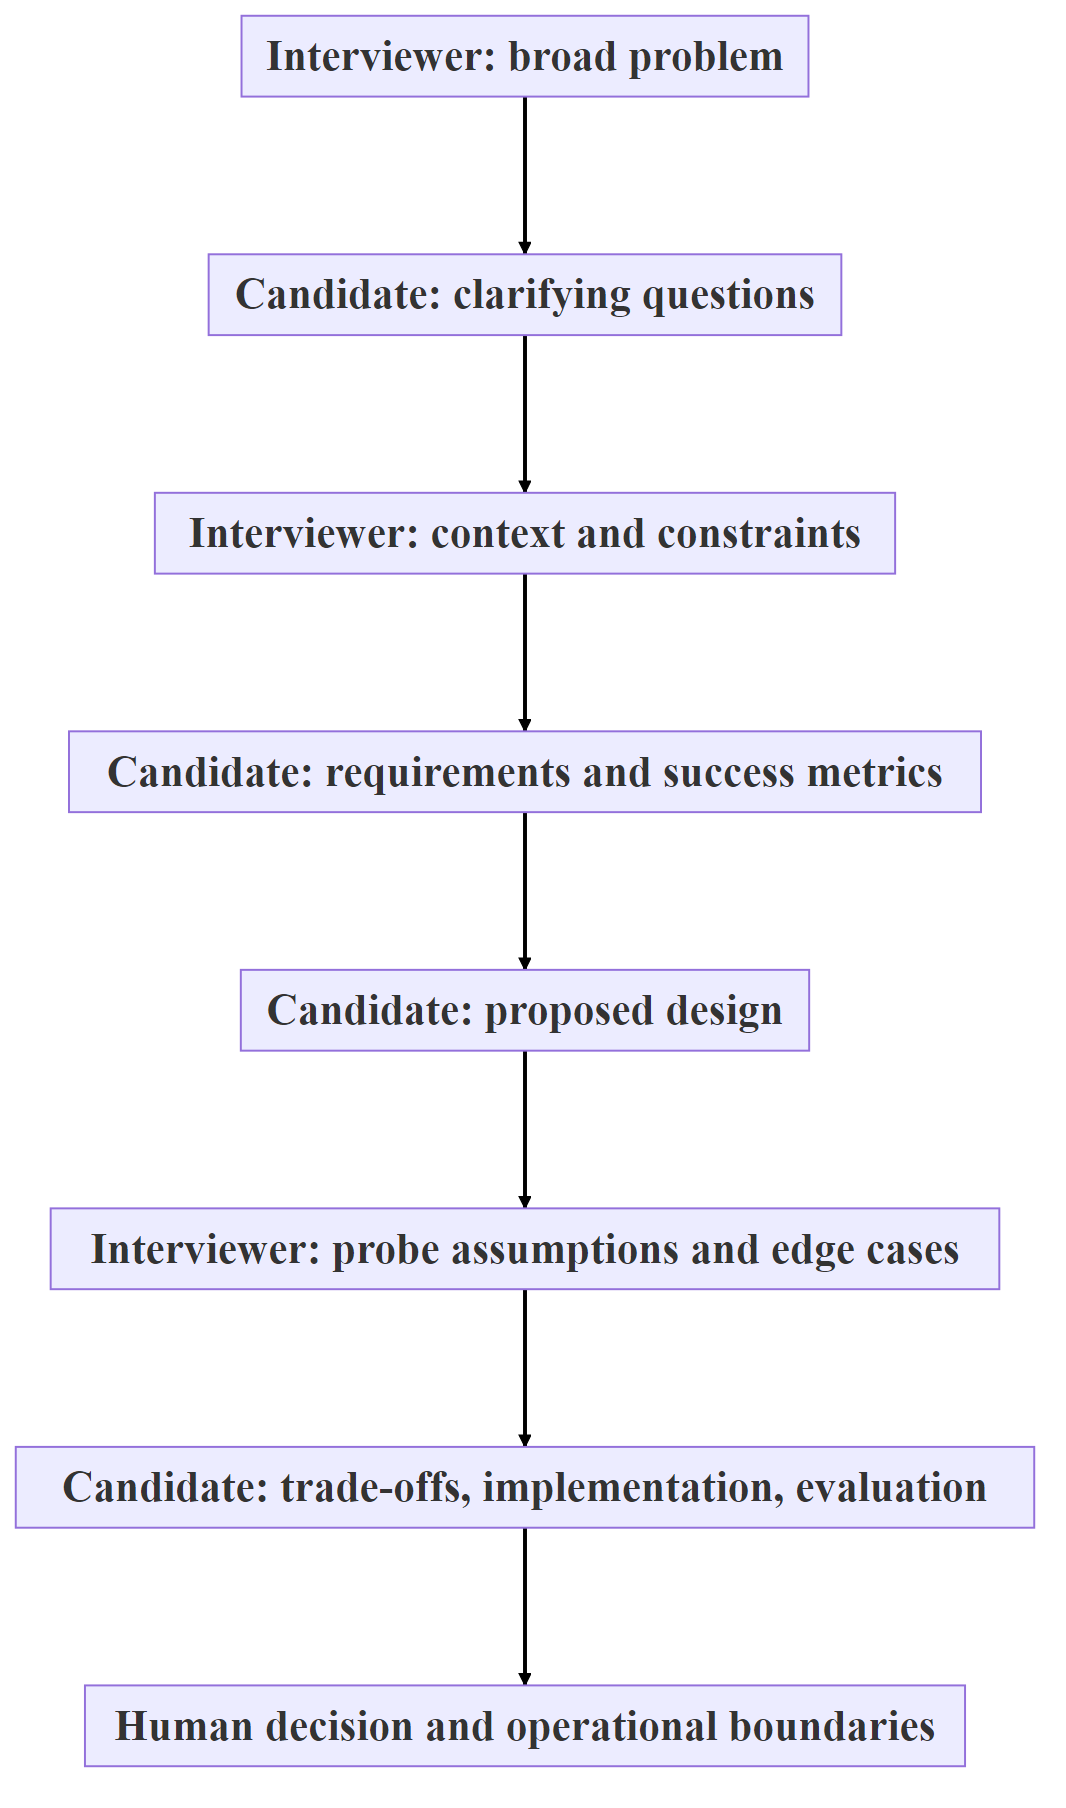
\includegraphics[width=\textwidth,height=0.85\textheight,keepaspectratio]{../diagrams/chapter_2_banking_foundations/06_flowchart_case-study-chapter-format.png}
\caption{Case-study chapter format}
\label{fig:ch02_banking_foundations-06-flowchart-case-study-chapter-format}
\end{figure}

This structure supports four kinds of readers. Consultants can practise discovery and solution framing. Freshers can see how business processes become data contracts and systems. Engineers can examine architecture, implementation choices, and failure handling. Interview candidates can practise turning a vague prompt into a structured answer without jumping immediately to a technology stack.

\subsection{Questions to keep asking}

\begin{itemize}
\item What is the actual business decision, and who is authorized to make it?
\item Which value is a source fact, which is a model extraction, and which is a deterministic calculation?
\item Which document, period, unit, customer, and version does this value belong to?
\item What happens when evidence is missing, contradictory, scanned, stale, or from the wrong entity?
\item Which parts are implemented in the described repository, and which are proposed enhancements?
\item Can a reviewer reproduce the output and see the exact reasons for an override?
\end{itemize}
The repeated lesson across all four studies is straightforward: useful AI in financial services makes evidence easier to find and explain, but it must preserve the institution's definitions, calculations, controls, and accountable decision-makers.
